\begin{figure}[t]
\centering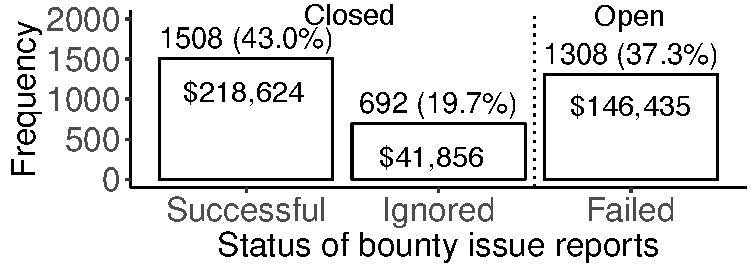
\includegraphics[width=0.8\columnwidth ]{pics/pre/pre_statusOfBounties.pdf}
\vspace{-0.1in}
\caption{The distribution of the possible statuses of bounty issue reports and their corresponding cumulative bounty value.}
\label{fig:pre_status_Bounties}
\vspace{-0.2in}

\end{figure}





In our preliminary study, we first present basic descriptive statistics
about the bounty: 1) the distribution of bounty issue reports across the possible statuses (i.e., successful, failed and ignored); 2) the distribution of the number of days between the reporting of the issue and its first bounty being proposed (i.e., \textit{days-before-bounty}); 3) the distribution of the frequency of bounties being used in projects (i.e., bounty-usage frequency).
From these statistics, we get a basic view of how bounties are used across projects. In addition, when a bounty issue report is closed and the bounty is paid out, we define this bounty issue report as addressed. We also calculate the issue-addressing likelihood against the bounty value and check the relationship between the issue-addressing likelihood and the bounty value.

%As we mentioned in Section~\ref{background}, in order to simplify our statement, we define three different bounties (i.e., the successful bounty, the failed bounty and the ignored bounty) according to three different status of the issue report.




\textbf{62.7\% of the bounty issue reports are closed, while the bounties in almost one-third of these closed issue reports remain unpaid with a value of \$41,856 in total.}
Figure~\ref{fig:pre_status_Bounties} shows the distribution of bounty issue reports across the three possible statuses. 37.3\% of the bounty issue reports are failed (i.e., open-unpaid). Although 62.7\% of the bounty issue reports were closed, almost one-third of their bounties were ignored (i.e., closed-unpaid). The total value of the ignored bounties (\$41,856) is ``frozen'' in the Bountysource platform unless someone claims the bounty.
In the rest of the paper, when we say the likelihood of an issue being addressed (i.e., issue-addressing likelihood), we only refer to the bounty issue reports that are successful (i.e., closed and paid out). We do not take the issue reports which were ignored into consideration because the hunters might not be driven by the bounty in such issue reports. We conducted a qualitative study of these closed-unpaid bounty issue reports to better understand them in Section \ref{rq4}.


\begin{figure}[t]
\centering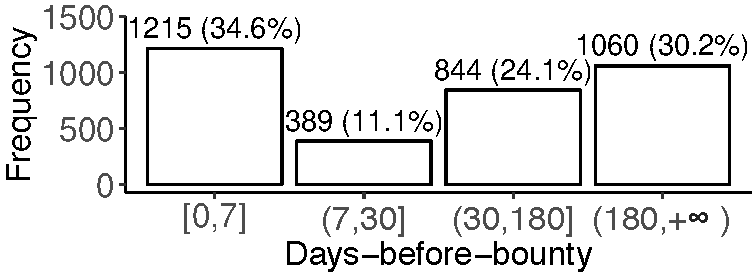
\includegraphics[width=0.8\columnwidth]{pics/pre/pre_delta_distribution_bounty}
\vspace{-0.1in}
\caption{The distribution of the number of days between the reporting of the issue and its first bounty being proposed (i.e., \textit{days-before-bounty}) in four different time ranges.}
\label{fig:pre_delta_distribution_bounty}
\vspace{-0.25in}

\end{figure}

\textbf{ 34.6\% of the bounties were proposed within 7 days from the creation of an issue report, while 30.2\% of bounties were proposed after more than 180 days.}
Figure~\ref{fig:pre_delta_distribution_bounty} shows the distribution of the \textit{days-before-bounty} metric in four continuous time ranges (i.e., 0 to 7 days, 8 days to 30 days, 31 days to 180 days, and more than 180 days). We observe that in 34.6\% of the issue reports their first bounty was proposed within 7 days after their creation, while in another 30.2\% of the issue reports their first bounty was proposed after more than 180 days since their creation.



 \begin{figure}[t]
   \centering
  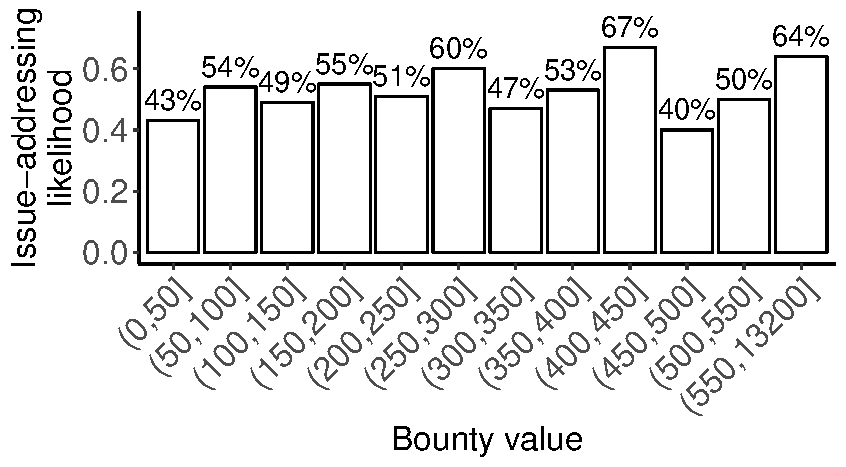
\includegraphics[width=0.8\columnwidth]{pics/pre/pre_i_value.pdf}
  \caption{The issue-addressing likelihood of the proposed bounty value ranges.}
  \label{fig:pre_v_value}
  \vspace{-0.1in}

\end{figure}

\textbf{More than half of the projects only used a bounty once, while two projects used bounties very frequently (more than 100 times)}. The distribution of the bounty-usage frequency of each project is skewed (with a variance of 57.02). 768 (65\%) projects used a bounty only once, 62 projects used a bounty at least 10 times and only 9 projects used a bounty more than 50 times.

%Because of the different bounty usage patterns in different projects, we investigate how the likelihood of an issue being addressed across projects with different bounty usage patterns in Section~\ref{rq1}.

%Figure~\ref{fig:preProjectEcdf} is the empirical cumulative distribution of the  bounty usage frequency for projects.



\textbf{The correlation between the bounty value and the issue-addressing likelihood is weak.} Figure~\ref{fig:pre_v_value} presents the issue-addressing likelihood of an issue report against the bounty value of an issue report. We do not observe patterns between them. The correlation between the bounty value and the issue-addressing likelihood is surprisingly weak~(0.14).

\rqbox{
Counter-intuitively, the correlation between the bounty value and the issue-addressing likelihood is weak. However, this low correlation may be due to the variation of the frequency of bounties that were used before in different projects and the timing of proposing the bounty.
}
Therefore, in Section~\ref{rq1} we investigate how the issue-addressing likelihood changes across projects with different bounty-usage frequencies. We study the relationship between the timing of proposing bounties and the issue-addressing likelihood in Section~\ref{rq2}.

